\chapter[REFERENCIAL TEÓRICO]{REFERENCIAL TEÓRICO}
\index{Referencial Teórico}
%\vspace*{-17mm}

Neste capítulo serão apresentados conceitos gerais do reconhecimento óptico de caracteres, bem como um pouco sobre cada uma das ferramentas usadas neste trabalho, em seguida serão detalhadas as características da base de áudios Braccent e ao final, há a descrição das métricas de comparação dos resultados.


\section{SISTEMAS DE TRANSCRIÇÃO}

Sistemas de transcrição da fala permitem que o computador interprete sinais de áudio, gerando transcrições textuais. 
De acordo com \citeonline{ferreira2017uso}, as arquiteturas clássicas de sistemas de transcrição tem quatro grandes componentes: modelo acústico, o modelo de linguagem, modelo léxico e decodificador. 

\begin{figure}[h!]
\centering
\caption{Arquitetura clássica de ASR.}
\label{fig:arqclassica}
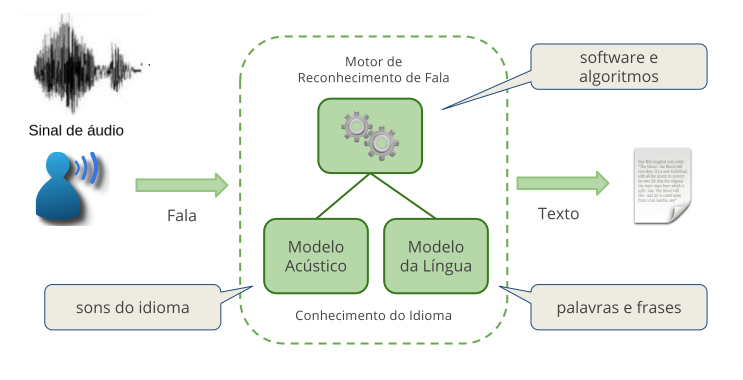
\includegraphics[width=130mm]{images/asr_2.png}
\fonte{\citeonline{cpqd}.}
\end{figure}

A \autoref{fig:arqclassica} apresenta a arquitetura com os componentes, onde o Modelo Acústico mapeia o sinal original que está sendo processado em palavras e sentenças; o Modelo da Língua é responsável por caracterizar a língua, a combinação de palavras e representa as palavras do dicionário com suas transcrições fonéticas; e Motor de Reconhecimento de Fala que é o  decodificador, que procura a melhor sequência de palavras possível. 



%Crescimento que provavelmente também foi impulsionado pela ``democratização da tecnologia'', através do livre acesso à essas tecnologias avançadas disponibilizadas pelos seus desenvolvedores
%O acesso é geralmente disponibilizado através de rotinas e padrões de programação, popularmente denominadas pela sigla API (\textit{Application Programming Interface}).  não passar pelo \textit{firewall}  da empresa,  endereço IP disponibilizado  via  DHCP por VM IP Static/global também estão disponíveis mas com custos adicionais),  Round-robin DNS para load balancing,, distribuição de carga geográfica (exemplo: Big-IP global traffic manager)

Na última década, as técnicas de aprendizado profundo começaram a ser utilizadas com sucesso em ASR \cite{dahl2011context}. Desde então, diversos sistemas comerciais começaram a se popularizar, principalmente os sistemas em nuvem. Devido a capacidade de escalabilidade e abstração, plataformas como serviço tem crescido praticamente 20\% ao ano \cite{krancher2018key}. 
A utilização destas ferramentas trazem vantagens, tais  como: elasticidade (rápida capacidade de escalabilidade), otimização de custos (devido ao compartilhamento de recursos),  virtualização  (fácil alocação  de  recursos), funcionalidades de operação e gestão, diferentes níveis de contratação,  VLANs privadas, controle de acesso dos endereços de IP e  compressão de conteúdo \cite{munteanumeeting}.
Grandes empresas da área tecnológica como IBM, Google, Microsoft, Amazon e Facebook já disponibilizaram serviços que utilizam inteligência artificial, sendo um deles o de transcrição. 

%conversor de voz para texto em que a inteligência artificial é utilizada para combinar as estruturas da linguagem e gramática com o processamento de sinais de voz, afim de obter uma identificação mais precisa das palavras. , fornecendo para diversos empreendimentos alta performance, segurança e confiabilidade em seus processos, otimizando a qualidade dos resultados adquiridos.

As ferramentas selecionadas para o desenvolvimento deste trabalho foram os das empresas Google e Facebook. 
A Google Cloud é uma plataforma mantida pelo Google, com  uma série de serviços na computação em nuvem, utilizado também pela própria empresa em produtos fornecidos ao usuário, como o Youtube. Diversos produtos são disponibilizados através dela, dentre eles podemos citar: processamento através de máquinas, armazenamento de objetos, serviço de banco de dados, processamento visual,  reconhecimento de fala e transcrição \cite{GoogleCloudGeral}. O serviço Speech-to-Text foi utilizado para realizar as transcrições dos áudios, onde uma rede neural é usada para o modelo de reconhecimento de voz com suporte a mais de 120 linguagens e dialetos. Apesar da utilização em geral ser paga, a plataforma fornece créditos válidos por um ano para iniciar o uso. \cite{kimura2018comparison}. 

%\subsection{Wit.ai}
A Wit.ai é mantida pelo Facebook e oferece aos desenvolvedores uma plataforma de linguagem natural que aprende a linguagem humana a partir de cada interação \cite{mitrevski2018getting}. Ao contrário da Google Cloud que é uma plataforma com diversas funcionalidades, a Wit.ai fornece apenas serviço de reconhecimento de fala e texto, sendo muito utilizada para a criação de \textit{chatbot} e reconhecimento da voz em aplicações. 

Para utilização é necessário realizar o login com uma conta do Facebook e não possui planos de uso, sendo totalmente gratuito com suporte para 132 linguagens e dialetos, porém uma de suas limitações é seu limite de tamanho de áudio, atualmente sendo de 20 segundos. Neste trabalho essa limitação não foi um problema, pois todos os áudios da base de dados possuem uma duração menor que o limite, com exceções de áudios que tiveram erros de gravação que foram removidos do escopo. \cite{WIT}.

\section{TRABALHOS CORRELATOS}

Nesta seção detalhamos dois artigos, um artigo de \citeonline{iinumaspeech} que faz uma comparação entre ferramentas da IBM, Google e Amazon para conversão de voz para texto de ligações telefônicas e um segundo artigo de  \citeonline{zelasko2018punctuation} que avalia a pontuação de transcrições de chamadas telefônicas.


Segundo \citeonline{iinumaspeech}, as tecnologias, ``Plataformas como serviço'', ``infraestrutura como serviço'' e ``Inteligência Artificial'',  estão sendo utilizadas para desenvolver sistemas que substituem pessoas em \textit{call centers}. Existindo casos até de fechamento completo de um \textit{call center} para trocar por uma \textit{startup} que utiliza programas de computador que substituem os seres humanos.
No artigo \cite{iinumaspeech} foram comparadas as ferramentas Google Cloud Speech to Text, IBM Watson Speech to Text e Amazon Transcribe. 

A base de dados foi composta de gravações de áudio com 6 (seis) diferentes interlocutores brasileiros que realizaram a leitura de uma parte do livro ``Divina Comédia''. São 3 (três) pessoas do sexo feminino e 3 (três) masculinos. Todos têm titulação de pós-graduação e faixa etária entre 40 e 50 anos. Foram realizados os seguintes pré-processamentos usando o aplicativo Audacity\footnote{https://www.audacityteam.org/}: eliminação de excesso de período sem falas, melhoria do volume e retirada de ruídos. 

%realizado uma pesquisa entre empresas influentes no âmbito tecnológico que disponibilizam serviços que utilizam inteligência artificial, sendo elas . Testando as suas ferramentas de conversão de voz para texto, 
Afim de comparar qual possui a melhor eficiência, foi usada a métrica de Taxa de Erros das Palavras (WER, do inglês \textit{Word Error Rate}). Para o WER, quanto menor o número, melhor será a qualidade do texto obtido. O WER é derivado da distância de Levenshtein, trabalhando no nível da palavra ao invés do nível do fonema. A partir da análise dos dados gerados pelo WER, constataram uma maior eficiência de conversão da API do Google (14,9\%), seguido pela API da IBM (15,23\%) e por último a API da Amazon (16,5\%), nota-se que a diferença entre as taxas de erro é baixa. É importante ressaltar que a pesquisa foi exploratória e as conclusões foram feitas com uma pequena base de experimentos (18 gravações no total) e uma pequena amostra de pessoas (6 pessoas).


% Em teoria, qualquer fonte de texto como blogs, artigos e Wikipédia poderiam ser utilizados como base de dados para realizar o treinamento da aplicação no uso de pontuação, porém a maioria deles não representam a linguagem coloquial. Portanto não dados fáceis de ser encontrados. 
%As redes neurais são treinadas na incorporação Common Web Crawl GloVe das palavras nas transcrições de Fisher alinhadas com os indicadores de conversação e informações de tempo de palavra. 

Em \citeonline{zelasko2018punctuation}, apresenta o problema de que muitos ASR não preveem pontuação ou capitalização. A falta de pontuação pode confundir tanto o leitor humano quanto os algoritmos de processamento de linguagem natural que usarão estes resultados. O texto sem pontuação além de poder ser confuso, pode ser difícil de ler, e algumas vezes perderem o real sentido do que foi dito. 
A proposta do trabalho foi o de treinar duas variantes de modelos de Rede Neural Profunda (DNN, do inglês \textit{Deep Neural Network}): a Memória de Curto-Prazo Longa Bidirecional (BLSTM, do inglês \textit{Bidirectional Long Short-Term Memory}) e uma Rede Neural Convolucional (CNN, do inglês \textit{Convolutional Neural Network}), para a predição de pontuação. 


Os modelos foram treinados no corpus inglês de Fisher \cite{cieri2004fisher}, que contém cerca de 11.000 conversas distintas com  anotações de pontuação. Foram considerados o tempo e duração de cada palavra, solução que até então não havia sido utilizado em outro sistema para realizar a tarefa de predição de pontuação. Nos experimentos, as transcrições de corpus de Fisher são alinhadas no tempo e pontuadas usando um algoritmo de alinhamento de sequência. Foram usadas 4 (quatro) classes de pontuação: espaço em branco (79,1\%), vírgula (11,5\%), ponto final (8,2\%) e ponto de interrogação (1,2\%). Os resultados são apresentados na \autoref{fig:pontos}.



A melhor acurácia foi com o modelo BLSTM considerando o alinhamento com o tempo das palavras. Pela matriz de confusão, o acerto do espaço (\textit{blank}) foi alta (0,95), mas não tanto para as demais pontuações. A CNN foi a que teve mais acertos nos caso de pontos de interrogação. As CNNs apresentam melhor precisão e os BLSTMs tendem a ter uma melhor revocação.  Os resultados constituem evidências significativas de que a distribuição de palavras no tempo podem ser úteis na tarefa de previsão de pontuação, pois apresentaram melhor resultado do que os modelos sem esta característica.


\begin{figure}[h!]
\centering
\caption{Matriz de confusão do melhor modelo BLSTM alinhado no tempo.}
\label{fig:pontos}
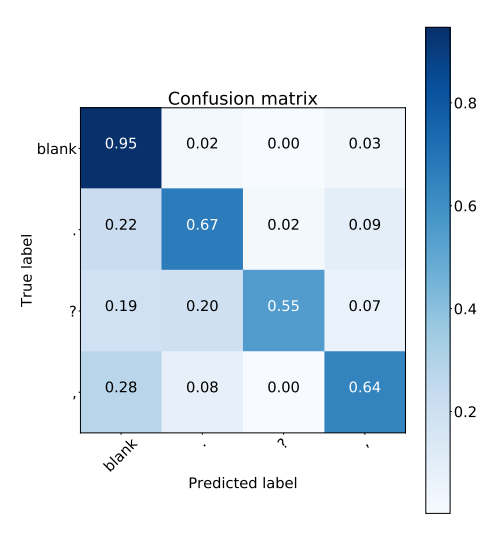
\includegraphics[width=0.5\textwidth]{images/matrzi.png}
\fonte{\citeonline{zelasko2018punctuation}.}
\end{figure}
%s cometam uma quantidade menor de erros no geral, a pontuação prevista pela CNN é mais precisa - especialmente no caso de pontos de interrogação. 

\section{BASE DE DADOS BRACCENT}

A base de dados Braccent foi criada por \citeonline{batista2019estudo}, e contém 1.743 amostras de fala. Há 7 sotaques brasileiros existentes na base, que são: nortista, baiano, fluminense, mineiro, carioca, nordestino e sulista. Os voluntários leem 16 sequências de frases, que foram criadas de forma a serem foneticamente balanceadas em seu conjunto e não necessariamente apresentam uma coerência semântica. O trabalho de origem da base de dados apresenta a  transcrição fonética, que foi realizada manualmente para cada sotaque regional pelos alunos do curso de Letras do ano de 2018 do Instituto de Estudos da Linguagem na Universidade Estadual de Campinas. O balanceamento fonético foi feito via análise da correlação de Spearman com a base Braccent e o CETENFolha\footnote{CETENFolha (Corpus de Extractos de Textos Eletrônicos NILC/Folha de S. Paulo) é um corpus de cerca de 24 milhões de palavras em português brasileiro, criado pelo projeto Processamento computacional do português com base nos textos do jornal Folha de São Paulo que fazem parte do corpus NILC/São Carlos, compilado pelo Núcleo Interinstitucional de Linguística Computacional (NILC).}, que foi de 89\%, maior que os 80\% do limiar descrito na literatura. Seguem as frases, com a pontuação e acentuação tal qual apresentado no trabalho original:

\begin{enumerate}[itemsep=3pt,parsep=3pt]
    \item Eu rasguei todo meu dinheiro em vão, minha família depende da aposentadoria do meu avô. Mas o dia amanheceu ensolarado e eu fiquei feliz porque minha tia viajou para Porto Alegre às sete horas.
    \item O telejornal da Globo terminou agora a pouco, todos se levantaram, a porta bateu forte e meu tio xingou bastante. Mas disse que é um grande prazer ter os sobrinhos hospedados em casa e não em um dos hotéis do sudoeste.
    \item Para ganhar, preciso decifrar o código até amanhã. Os papeis foram rasgados mas ainda é possível ler informações importantes.
    \item Suas atitudes são muito drásticas e resultarão em guerra entre vocês. Ela chegou a pedir o divórcio antes dele morrer e pensou que podia compartilhar esse documento com você.
    \item Meu orientador disse que o professor de Português e a professora de Matemática se casaram e foram morar na Nigéria, onde o clima está muito diferente de dez anos atrás.
    \item Você tem razão, a correção da prova não foi justa e a turma tirou notas abaixo da média. Assim como a gestão do atual prefeito, a diretoria não está agradando o povo.
    \item Tenho aptidão para tirar fotos de motos e guitarras, então recebi em dólar e comprei um carro, jóias e relógios para nós. A atriz teve uma ótima atuação no espetáculo e recebeu meus parabéns e um presente pela apresentação fantástica.
    \item Eu criei muita expectativa nesse trabalho. O chefe não ouviu meu clamor, continuou sorrindo para mim e segurando a colher que estava suja de abacate ele disse ``A palavra caçador se escreve com C cedilha''.
    \item O Brasil é um país injusto e desigual, é errado não partilhar a comida com os mais necessitados. Mas só vota quem tiver o título de eleitor.
    \item Esse canal tem bastante pornografia e a abertura do campeonato ocorreu antes de ontem, quando os turistas japoneses procuravam belas casas para alugar.
    \item O biscoito era de chocolate com morango, por isso escolhi o bombom de chocolate ao leite com licor de Amarula. Ainda precisamos comprar pó de café, pão francês, abóbora e melão.
    \item Segurei a panela de macarrão com apenas uma mão e as duas pilhas que eu lhe dei caíram no chão. A rã está embaixo do fogão, deve ser retirada logo, pois tenho medo de répteis e de minhocas.
    \item Ele pulou daquele caminhão que transportava tubos de ferro e nega que naquela área tem produtos tóxicos. Foi na cidade em que encontraram o corpo do mendigo numa bocada e montaram uma emboscada para prender os assaltantes. 
    \item Ele ficou chateado porque foi chamado de burro pelo escrivão zangado enquanto lavava sua blusa azul de lã com água e sabão.
    \item Li que o escrivão mora sozinho perto da plantação de feijão e sorte que o jacaré que fugiu do zoológico já foi encontrado.
    \item A velha locomotiva vem com pouca carga e os faróis iluminam as flores da rua em que a criança desenhou um vulcão.
\end{enumerate}


As gravações são identificadas de acordo com o gênero e o sotaque regional falado na locução, sendo 872 amostras do sexo feminino e 871 amostras do sexo masculino, conforme distribuição da Tabela \ref{tab:tabBraccent}. É possível verificar pela tabela que há desbalanceamento quanto à quantidade de áudios por sotaque, com muito mais exemplares do sulista enquanto há poucos nortistas.  Foram 142 locutores com diferentes faixas etárias e níveis de escolaridade, e a quantidade de áudio de cada locutor variou entre 1 e 16. 

\begin{table}[h!]
\centering
\caption{Descrição do Número de Gravações da Base de Dados Braccent.}
\label{tab:tabBraccent}
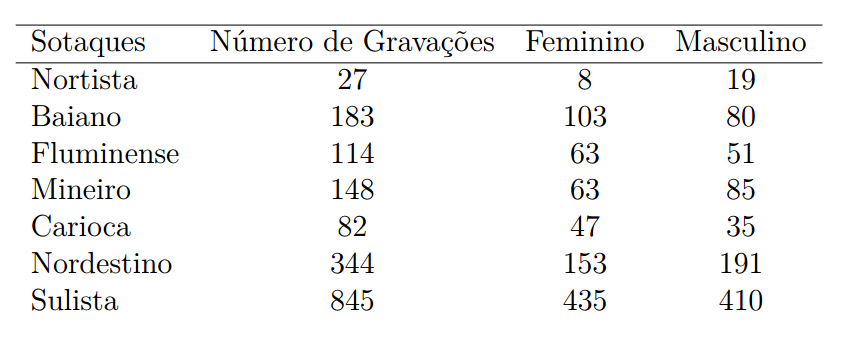
\includegraphics[width=0.6\textwidth]{images/tabBraccent.png}
\fonte{retirado de \citeonline{batista2019estudo}}
\end{table}



\section{MÉTRICAS DE COMPARAÇÃO}

Neste trabalho foi utilizado a métrica de Levenshtein Distance para analisar o desempenho das API's. A distância de Levenshtein foi introduzida em 1995 por Kessler para medir a distância entre dialetos \cite{kessler1995computational}. Dada pelo número mínimo de operações necessárias para transformar um trecho no outro. Existindo três tipos de operações para realizar o processamento: inserção, exclusão e substituição de caracteres \cite{beijering2008predicting}.

Seu funcionamento ocorre pelo preenchimento de uma matriz (n) x (m), na qual n e m são o número de caracteres das duas \textit{strings} a serem comparadas. Como exemplo, vamos comparar as \textit{strings} ``TESTE'' em ``TECLA'', que origina uma matriz 5 x 5, conforme \autoref{LevenshteinPasso1}. 

\begin{quadro}[h]
\caption{Passo inicial da execução da métrica de Levenshtein}
\label{LevenshteinPasso1}
\centering
\begin{tabular}{cc|c|c|c|c|c|}
\textbf{}  & \textbf{} & \textbf{T} & \textbf{E} & \textbf{S} & \textbf{T} & \textbf{E} \\ 
\textbf{}  & 0         & 1          & 2          & 3          & 4          & 5          \\ \hline
\textbf{T} & 1         &            &            &            &            &            \\ \hline
\textbf{E} & 2         &            &            &            &            &            \\ \hline
\textbf{C} & 3         &            &            &            &            &            \\ \hline
\textbf{L} & 4         &            &            &            &            &            \\ \hline
\textbf{A} & 5         &            &            &            &            &            \\ \hline
\end{tabular}
\fonte{elaborado pelo próprio autor (2021)}
\end{quadro}

\begin{quadro}[h!]
\caption{Passo intermediário da execução da métrica de Levenshtein}
\label{LevenshteinPasso2}
\centering
\begin{tabular}{cc|c|c|c|c|c|}
\textbf{}  & \textbf{} & \textbf{T} & \textbf{E} & \textbf{S} & \textbf{T} & \textbf{E} \\ 
\textbf{}  & 0         & 1          & 2          & 3          & 4          & 5          \\ \hline
\textbf{T} & 1         & 0          & 1          &           &           &           \\ \hline
\textbf{E} & 2         &     1       &      0      &            &            &            \\ \hline
\textbf{C} & 3         &            &            &            &            &            \\ \hline
\textbf{L} & 4         &            &            &            &            &            \\ \hline
\textbf{A} & 5         &            &            &            &            &            \\ \hline
\end{tabular}
\fonte{elaborado pelo próprio autor (2021)}
\end{quadro}
\begin{quadro}[h]
\caption{Passo final da execução da métrica de Levenshtein}
\label{LevenshteinPasso3}
\centering
\begin{tabular}{cc|c|c|c|c|c|}
\textbf{}  & \textbf{} & \textbf{T} & \textbf{E} & \textbf{S} & \textbf{T} & \textbf{E} \\ 
\textbf{}  & 0         & 1          & 2          & 3          & 4          & 5          \\ \hline
\textbf{T} & 1         & 0          & 1          & 2          & 3          & 4          \\ \hline
\textbf{E} & 2         & 1          & 0          & 1          & 2          & 3          \\ \hline
\textbf{C} & 3         & 2          & 1          & 1          & 2          & 3          \\ \hline
\textbf{L} & 4         & 3          & 2          & 2          & 2          & 3          \\ \hline
\textbf{A} & 5         & 4          & 3          & 3          & 3          & 3          \\ \hline
\end{tabular}
\fonte{elaborado pelo próprio autor (2021)}
\end{quadro}
%, pois em todas comparações pelo menos uma das \textit{strings} é vazia. Portanto a única operação que é realizada é de inclusão de caractere até formar a outra \textit{string}. A posição (1,1) começa com 0 (zero). 
Dando início ao preenchimento das células restantes, existem duas possibilidades que devem ser observadas para realizar o preenchimento. Devemos verificar se as  \textit{substring} são iguais ou não. Analisando a célula (1,1), deve-se comparar os caracteres 'T' e 'T', nesse caso o campo é preenchido com o valor 0 (zero), pois são iguais. Como os caracteres adicionados em cada \textit{substring} são os mesmos, a matriz é transposta. %não é necessário realizar nenhuma operação extra, portanto seu valor é igual a diagonal superior esquerda, que representa o resultado das mesmas Strings desconsiderando ambos caracteres.

Avançando um caractere, compara-se as \textit{substrings} ``T'' com ``TE'' para a posição (1,2), a comparação de ``TE'' com ``T'' para a posição (2,1) e comparação de ``TE'' com ``TE'' para a posição (2,2). Cada célula é preenchida da seguinte forma: à esquerda (custo da inclusão), acima (custo da exclusão) e na diagonal (custo da substituição). O custo de inclusão é 1, o custo de exclusão é 1 e o custo de substituição é 0 (são iguais).

%da célula atual e então é somado um ao valor encontrado. Na posição (1,2) da matriz, os últimos caracteres da \textit{substring} são diferentes ('T' e 'E'), portanto Portanto a terceira célula da segunda linha deve ser preenchido com o valor 1.


Continua-se o preenchimento dos campos restantes seguindo o processo explicado anteriormente. Na próxima comparação, \textit{substrings} ``TEC'' e ``TES'', na diagonal (3,3) o valor é 1, pois deve-se substituir um caractere. E os custos de inclusão (células na linha até a diagonal ou células à esquerda) e exclusão (células na coluna até a diagonal ou células acima) são preenchidos. Ao final, a matriz fica como mostrado no  \autoref{LevenshteinPasso3}. 

Cada célula da matriz representa o custo mínimo para transformar a respectiva parte da \textit{string} na outra, portanto, a última célula da matriz representa o valor mínimo para transformar a \textit{string} ``TESTE'' em ``TECLA''. A posição (5,5) é o resultado da distância de  Levenshtein, que é o custo mínimo para transformar ``TESTE'' em ``TECLA'', que são 3 operações, de acordo com o algoritmo.



Além do Levenshtein, foi utilizado Levenshtein Normalizado, que é obtido através da divisão do valor da distância Levenshtein pelo tamanho da maior \textit{string}, resultando em um valor percentual da proximidade entre as duas \textit{strings}. Utilizando o exemplo anterior, o Levenshtein Normalizado teria como resultado 0,6 (3 dividido por 5), logo, 60\% de semelhança entre as duas \textit{strings}.


